%%%Preamble
\documentclass[12pt]{article}
\usepackage{epsfig, amsfonts, cite, amssymb}
\usepackage{subfigure}
\usepackage{array}
\usepackage{float}
\usepackage{enumitem}
\usepackage{indentfirst}
\usepackage{boldline}
\usepackage[usenames,dvipsnames,svgnames,table]{xcolor}
\usepackage{amsmath}

%%% Use these when running Text Verifications
%\usepackage[T1]{fontenc}        
%\usepackage[utf8]{inputenc}     
%\usepackage[adobe-utopia]{mathdesign}
%\usepackage{printlen}

\voffset=0in \hoffset=0in \textwidth=6.3in \textheight=8.3in
\setlength{\oddsidemargin}{0in} \setlength{\textwidth}{6 in}
\thispagestyle{empty}

\begin{document}

\begin{figure*}[htb]
\subfigure{
\includegraphics[width=2.5in]{wne.eps} }
\hfil \hspace{.5in}
\subfigure{
\includegraphics[width=2.5in]{department.eps} }
\end{figure*}

%%%Header
\begin{center}
{\Large {\bf CPE 462/562 VHDL: Simulation \& Synthesis}}\\
\vspace{0.2in}
{\Large{Midterm Project: 4-bit ALU Design and Implementation}} \\
\vspace{0.2in}

%%%Cover Page
Katelyn Charbonneau\\
Email: kc325844@wne.edu\\
Date: 10/27/2017\\
\end{center}

\begin{table}[!h]
\centering
\begin{tabular}{| >{\arraybackslash}m{4in} | >{\centering\arraybackslash}m{1in} | }
  \hline
  % after \\: \hline or \cline{col1-col2} \cline{col3-col4} ...
  \textbf{Tasks} & \textbf{Grades} \\
  \hline
  &\\
  Task 1. Design, test, and verify 4-bit ALU (50') & \\
  &\\
  \hline
  &\\
  Task 2. Program DE2-115 and demonstrate 4-bit ALU (10') & \\
  &\\
  \hline
  &\\
  Task 3. Display INPUT and OUTPUT decimal equivalent values on SSDs (20') & \\
  &\\
  \hline
  &\\
  Report (20') & \\
  &\\
  \hline
    &\\
  Bonus (10') & \\
  &\\
  \hline
  \hline
    &\\
  \textbf{Total (100/110):} & \\
  &\\
  \hline

\end{tabular}
\label{table_cover}
\end{table}

%%%Text Verifications
%This text is \fontname\font\ with font size \csname f@size\endcsname{}
%and \verb|\baselineskip| =~\the\baselineskip =~\uselengthunit{mm}\printlength{\baselineskip}.

%%% END of Cover Page
\newpage

\section{Objective} \label{sec:obj}
The objectives of the project are to be familiar with behavioral architecture; be able
to write a behavioral VHDL code to design a 4-bit arithmetic logic unit (ALU), write
a testbench to verify the design, and implement the ALU on FPGA.

\section{Design Procedure} \label{sec:desproc}
The top level design block is shown in Figure \ref{fig:toplevel}.

\begin{figure}[!h]
\setlength{\belowcaptionskip}{-10pt}
\begin{center}
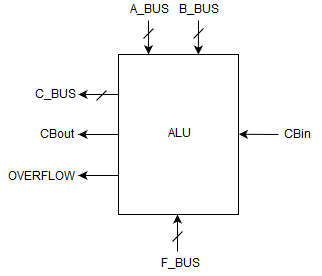
\includegraphics[scale=0.5]{ALU_top_level.png}
\caption{ALU Top Level Block}
\label{fig:toplevel}
\end{center}
\end{figure}

Where A\textunderscore BUS, B\textunderscore BUS, and C\textunderscore BUS are SIGNED(N-1 DOWNTO 0), F\textunderscore BUS is STD\textunderscore LOGIC\textunderscore VECTOR(2 DOWNTO 0), and CBin, CBout, and OVERFLOW are STD\textunderscore LOGIC.

\vspace{14.5pt}

The operations that the ALU can perform, as listed in the project requirements, are listed below:

\begin{table}[!ht]
\vspace{0.1in}
\centering
	\rowcolors{2}{gray!10}{white}
	\begin{tabular}{ c  c  c  c} %\cline{2-7}
	\hlineB{4}
	\rowcolor{gray!25}
	\textbf{F\textunderscore BUS} & \textbf{C\textunderscore BUS} & \textbf{CBout} & OVERFLOW\\\hlineB{4}
	000 & A\textunderscore BUS & PASS & 0\\\hline
	001 & A\textunderscore BUS + B\textunderscore BUS + CBin & CBout & Overflow \\\hline
	010 & A\textunderscore BUS - B\textunderscore BUS - CBin & CBout & Overflow\\\hline
	011 & A\textunderscore BUS \textit{OR} B\textunderscore BUS & PASS & 0\\\hline
	100 & A\textunderscore BUS \textit{XOR} B\textunderscore BUS & PASS & 0\\\hline
	101 & A\textunderscore \textit{SRA} 3 & PASS & 0\\\hline
	110 & A\textunderscore BUS \textit{SLL} 2 & A\textunderscore BUS(N-1) & Overflow\\\hline
	111 & A\textunderscore BUS \textit{ROR} -3 & PASS & 0\\\hlineB{4}
	\end{tabular}
\label{tab:operations}
\caption{ALU Operations}
\end{table}

\newpage

While testing of this design was done using a 4-bit bus width, their sizes are really defined as generics.  Thus, there is a variable bus size.  As part of this project, a ripple carry adder (RCA) is needed.  A fixed 4-bit width RCA design was available and was edited to also allow for a variable bus width.  This design was tested using a 6-bit width; sample results are in Section \ref{simresults}.	A block diagram for this is shown in Figure \ref{fig:rca}.

\begin{figure}[H]
\setlength{\belowcaptionskip}{-10pt}
\begin{center}
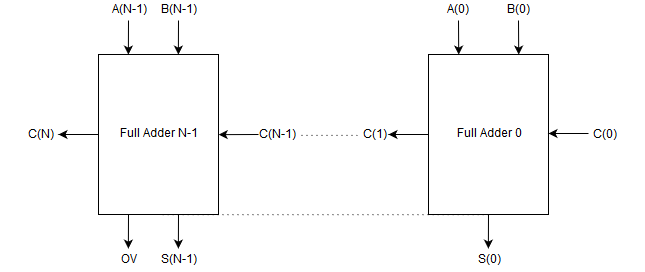
\includegraphics[scale=0.6]{Scalable_rca.png}
\caption{The RCA used to perform arithmetic calculations}
\label{fig:rca}
\end{center}
\end{figure}

Where N is the bus width, A, B, and S (sum) are signed vectors of length N-1, C (carry) is a standard logic vector of length N, and OV is defined as C(N) $\oplus$ C(N-1).

\vspace{14.5pt}

The RCA is used in cases 1 and 2 - addition and subtraction.  A CBout of "PASS" simply passes the value of CBin through.  For subtraction, the complement of B\textunderscore BUS is taken. All other cases are handled by simple pre-defined operations within VHDL.   Note that there is overflow for case 6 if the value of A\textunderscore Bus(N-1) changes after shifting.\par
In addition to this basic functionality, additional output ports had to be defined to accommodate implementation onto the FPGA.  Inputs and outputs are displayed on both LEDs and seven-segment displays.  A previously used design for these displays was re-used as a component.  The third component used in the project described behavior for the negative signs that lit up only when the associated bus decimal value was negative.

\newpage

\section{Simulation Results} \label{simresults}

\begin{figure}[H]
\begin{center}
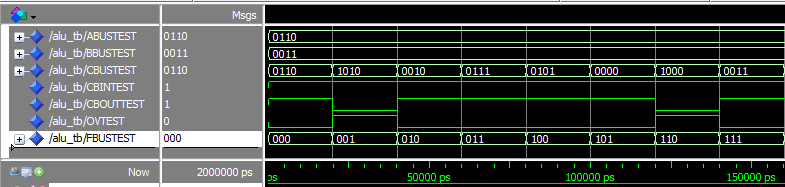
\includegraphics[scale=0.7]{ALU_sim.png}
\caption{Sample simulation results for the ALU}
\label{fig:simalu0}
\end{center}
\end{figure}

\begin{figure}[H]
\begin{center}
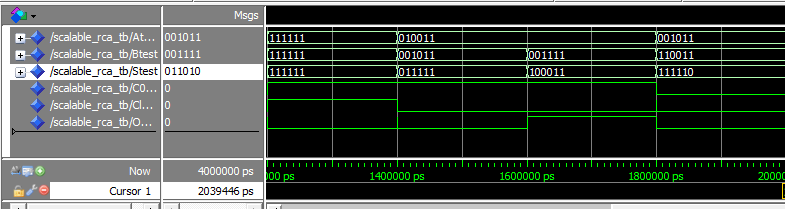
\includegraphics[scale=0.7]{rca_sim_results_example.png}
\caption{Operations on the RCA design showing variable bus width functionality}
\label{fig:simrca0}
\end{center}
\end{figure}

\newpage

\section{Demonstration on FPGA} \label{demo}
The design was synthesized onto the Altera Cyclone IV E DE2-115F29C7 FPGA.
\begin{itemize}
\item User Controls:
	\begin{itemize}
	\item Input A: Switches 3 down to 0
	\item Input B: Switches 8 down to 5
	\item Operation Select: Switches 15 down to 13
	\item Carry/Borrow in: Switch 17
	\end{itemize}
\item Input and Output Displays:
	\begin{itemize}
	\item Inputs
		\begin{itemize}
		\item A: Hex displays 7 and 6
		\item B: Hex displays 5 and 4
		\item Carry/Borrow in: Green LED 8
		\end{itemize}
	\item Outputs
		\begin{itemize}
		\item C: Green LEDs 3 down to 0, as well as hex displays 1 and 0
		\item Carry/Borrow out: Green LED 5, as well as hex display 2
		\item Overflow: Green LED 7, as well as hex display 3
		\end{itemize}
	\end{itemize}
\end{itemize}

\begin{figure}[H]
\begin{center}
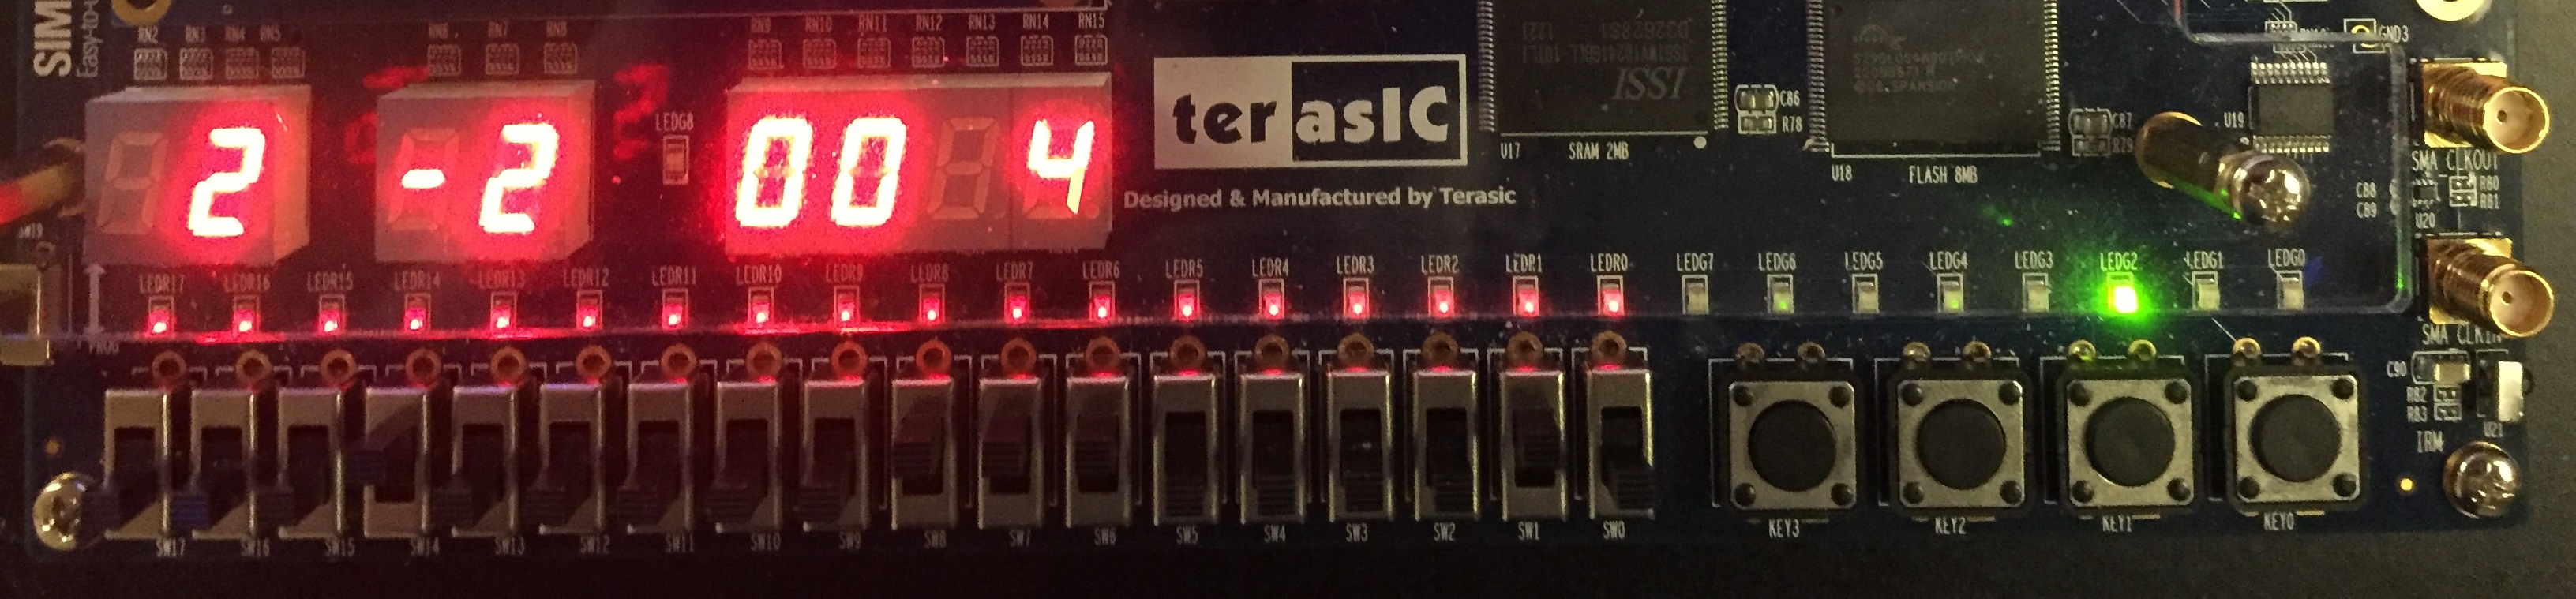
\includegraphics[scale=0.1]{example_subtraction.png}
\caption{Subtraction of decimal 2 - (-2) = 4}
\label{fig:boardsim0}
\end{center}
\end{figure}

\begin{figure}[H]
\begin{center}
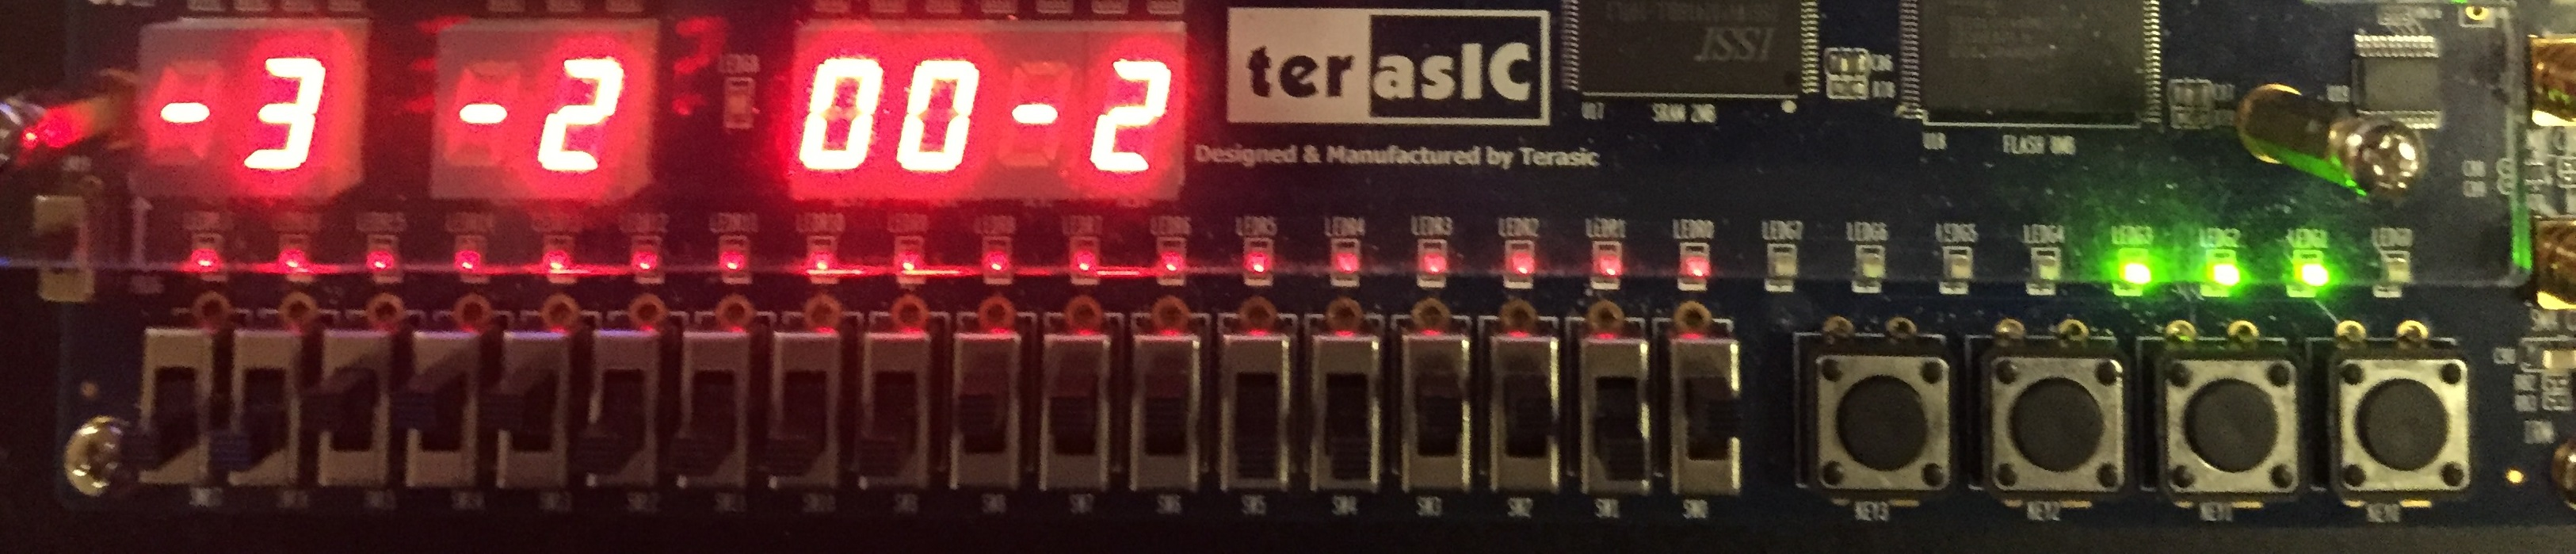
\includegraphics[scale=0.1]{example_rotate.png}
\caption{Rotate operation 1101 -> 1110}
\label{fig:boardsim1}
\end{center}
\end{figure}

\begin{figure}[H]
\begin{center}
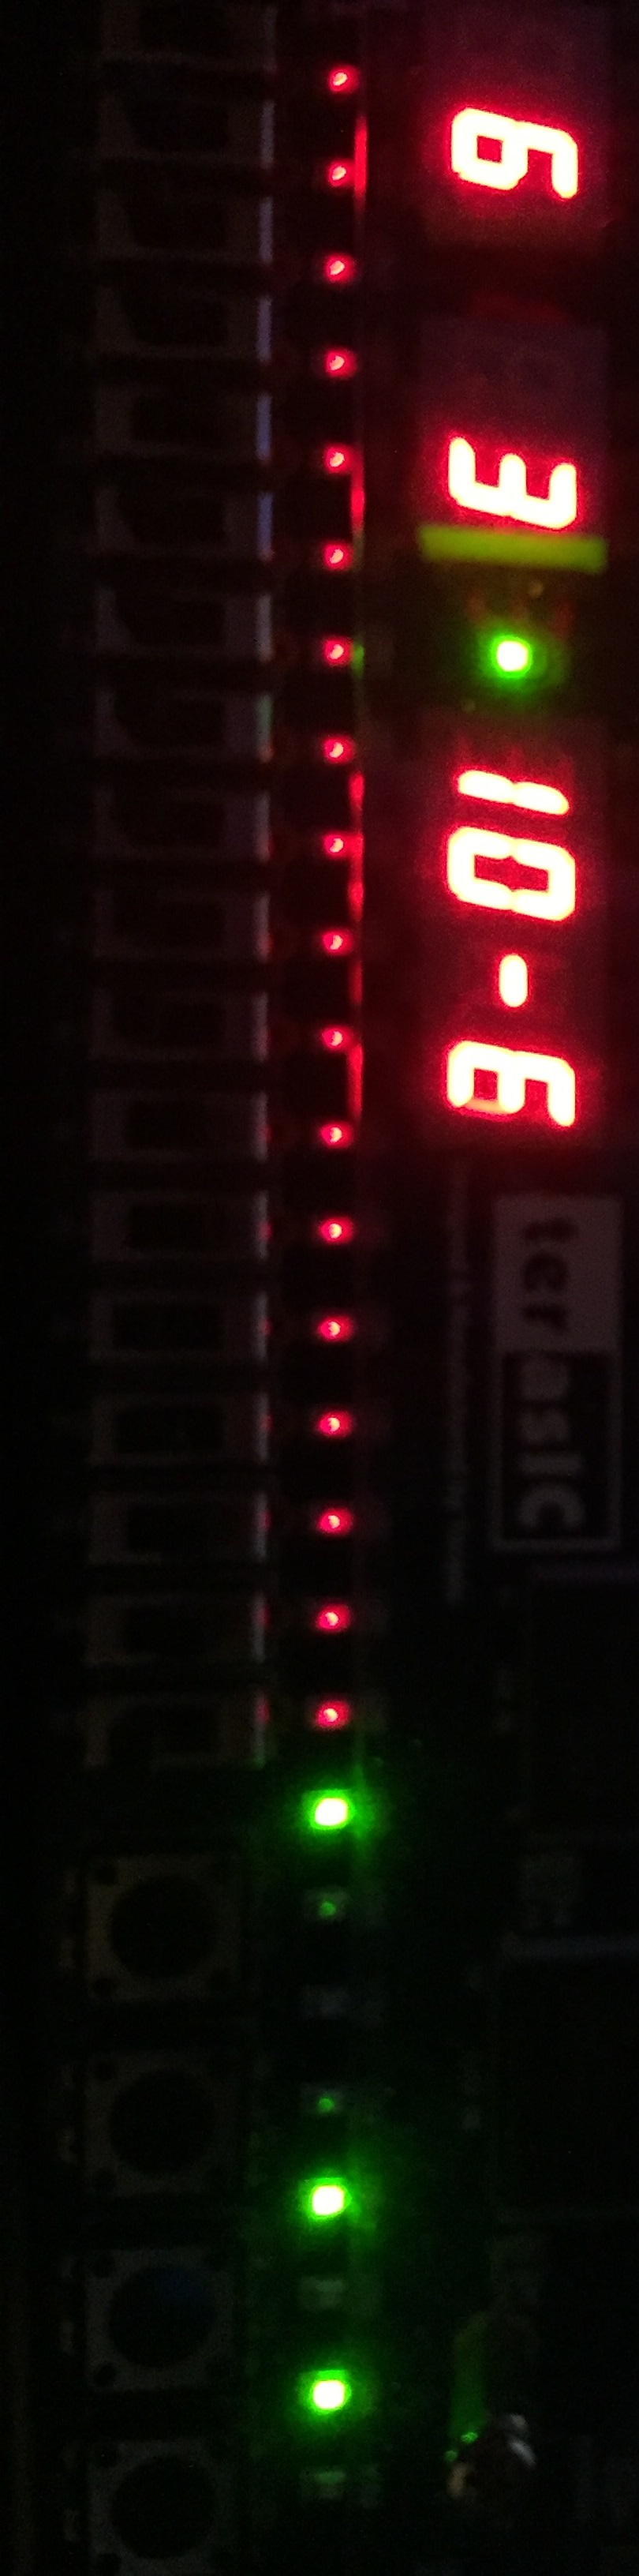
\includegraphics[scale=0.1, angle=90]{example_inthedark.png}
\caption{Addition of 3 + 6 with overflow; in dark to show visibility differences}
\label{fig:boardsimdark}
\end{center}
\end{figure}

\section{Conlusion} \label{cncl}
The project simulated and synthesized correctly.  The code required sufficient knowledge of structural and concurrent VHDL.  Multiple lower-level components were used and many concurrent statements were utilized.  Generics were used on multiple levels to allow the size of the ALU to be changed easily, however, the implementation onto the FPGA relied upon a bus width of 4 bits.  As such, it could be quite difficult to really change the size as-is.  While the size is changeable from  just a few constants, more work would need to be done to make it truly scalable.

\end{document} 
